\documentclass{article}

% if you need to pass options to natbib, use, e.g.:
%     \PassOptionsToPackage{numbers, compress}{natbib}
% before loading neurips_2019

% ready for submission
% \usepackage{neurips_2019}

% to compile a preprint version, e.g., for submission to arXiv, add add the
% [preprint] option:
%     \usepackage[preprint]{neurips_2019}

% to compile a camera-ready version, add the [final] option, e.g.:
     \usepackage[final]{neurips_2019}

% to avoid loading the natbib package, add option nonatbib:
%     \usepackage[nonatbib]{neurips_2019}

\usepackage[utf8]{inputenc} % allow utf-8 input
\usepackage[T1]{fontenc}    % use 8-bit T1 fonts
\usepackage{hyperref}       % hyperlinks
\usepackage{url}            % simple URL typesetting
\usepackage{booktabs}       % professional-quality tables
\usepackage{amsfonts}       % blackboard math symbols
\usepackage{nicefrac}       % compact symbols for 1/2, etc.
\usepackage{microtype}      % microtypography
\usepackage{graphicx}

\title{Comparison of Dimensionality Reduction Techniques}

\author{%
  Jonathan Tan \\
  Harris School of Public Policy\\
  University of Chicago\\
  Chicago, IL 60637 \\
  \texttt{jonathantan@uchicago.edu} \\
  \And
  Satej Soman \\
  Harris School of Public Policy\\
  University of Chicago\\
  Chicago, IL 60637 \\
  \texttt{satej@uchicago.edu} \\
}

\begin{document}

\maketitle

\begin{abstract}
  We compare two dimensionality-reduction techniques: principle components analysis (PCA) and latent space representation via autoencoder neural networks. Both techniques are applied to a feature set and the reduced feature-set is used as the independent variables in a linear regression to recover a known score. We find that autoencoders with sigmoid activations outperform both PCA and ReLU-activation neural networks for this dimensionality reduction task. 
\end{abstract}

\section{Background}
Dimensionality reduction is an important technique to render high-dimensional datasets more tractable for analysis. Often, in a dataset containing thousands of columns, a small number of those columns are relevant for an analytical task. Robust techniques for identifying the most salient features allow for more compact representations of data, reducing storage costs and analysis time [1], [2].

\section{Techniques studied}
\subsection{Principal components analysis}
Principal component analysis is a dimensionality reduction technique built upon the singular value decomposition (SVD) of a feature matrix. Specifically, the SVD produces matrices $X = U \Sigma V^T$ such that the right singular vectors of $X$, i.e. the columns of $V$, give the principal component directions of $X$. We can obtain a lower-dimensional representation of the original features by projecting the data onto the first $n$ principal component directions.[3]. Below, we vary the number of principal components used to predict wine scores and observe how mean squared error between predicted and true wine scores vary with $n$.

A known limitation of PCA is that it is not particularly effective at detecting and representing nonlinear relationships in the data. Thus, we are interested in exploring dimensionality reduction techniques that address this limitation.
\subsection{Autoencoders}
In contrast, autoencoders seek to map inputs to a \emph{non-linear} input manifold. An autoencoder is an artificial neural network that seeks to learn a compressed representation of its input [1], [4], [5]. Generally, an autoencoder has two stages: a number of encoding layers that reduce the dimension of the input vectors, and a number of decoding layers that attempt to reconstruct the original input from the latent representation. Our networks focus on the encoding step since we are interested in the latent representation.

All of our autoencoders produced output vectors of length 50. We trained neural networks with three main architectures. The shallowest was simply a 50-layer hidden layer in between an input and output layer. The deeper networks we tested progressively stepped the input size down. Most of our architectures had only a single decoding layer. We also tested networks where all layers had the same activation function (either sigmoid or ReLU), as well as an architecture where all hidden and input layers had ReLU activation, feeding into an output layer with sigmoid activation.

To train the networks, we used stochastic gradient descent over a variable number of training epochs. To maintain decoded fidelity, our output node delta for the update step was proportional to the difference in input and output vectors [6].
\section{Dataset decription and feature generation}
We use a dataset of wine reviews from Kaggle [7] consisting mostly of categorical and text data, each with an associated wine review score on a scale of 80 - 100. The features include a free-text description of the wine, as well as pre-parsed information about the wine, including type, grape variety, region of origin, and winery. The key continuous, numeric column in the feature set is the price of each wine bottle. The label we seek to recover is the wine review score.

Much of the Kaggle dataset is text or categorical data. Specifically, the “description” feature contains paragraph text of descriptors for each wine. To obtain a numeric representation of this text data, we used a simple boolean bag-of-words model. We first preprocessed the text data by converting all words to lowercase, removing non-alphanumeric characters and common stopwords, then tokenizing the space-delimited string into separate words. Lastly, we computed a bit vector for each row that represented a one-hot encoding for each word in the description, over all unique words in all rows of the description feature.

The bag-of-words model gives a particularly sparse matrix, and we faced initial difficulties in computing the representation with the full 130,000-row dataset (which had roughly 45,000 unique tokens). Specifically, the resulting matrix from the description column alone was over 100GB and, when the process ran in a reasonable amount of time, we had difficulty storing the data on our local machines. As an interim solution, we proceeded with a reduced dataset, taking 10,000 rows from the wine dataset instead. 

\section{Methodology}
For each technique, we apply the dimensionality reduction to obtain a reduced set of feature vectors ($X_j$). We then regress wine score ($S_i$) on these reduced features to estimate the least squares weights for the reduced feature set and then calculate predicted scores from the learned weights. Finally, we compare the mean-squared error arising from the true vs. predicted wine scores for several dimensionality reduction techniques.

\section{Results}
Table \ref{msetable} shows the resulting mean-squared errors for each dimensionality technique we studied, along with a description of each technique. For PCA runs, we report the number of principal components used in regression. For autoencoders, we report the architecture (shallow: 1 hidden layer, medium: 3 hidden layers, deep: 5 hidden layers), the activation function (ReLU or sigmoid), and the number of epochs used to train the network. There are two special networks: one ReLU network with a sigmoid output layer, and a completely symmetric network with the same number of encoding and decoding layers. 

As the table indicates, the sigmoid autoencoder performed the best, followed by PCA with a reasonable number of components, and then ReLU autoencoders. The special architectures described above did not improve performance.

Figures \ref{msek}, \ref{aenn_sigmoid}, and \ref{aenn_relu} investigate the performance of each technique in more detail. As seen in Figure \ref{msek}, MSE drops very quickly as the number of included principle components increases but levels off after approximately 5 or so included components. This indicates the ideal \emph{linear} representation of the data is captured by those components.

Figures \ref{aenn_sigmoid} and \ref{aenn_relu} look at the neural networks' performance. Surprisingly, the number of epochs we trained the network for had no effect on MSE. Additionally, the shallow architectures outperformed the deeper ones, while sigmoid activation was orders of magnitude more performant than ReLU activation.

\begin{table}
    \centering\small
\begin{tabular}{llr}
\toprule
     technique &                     description &          MSE \\
\midrule
autoencoder &   sigmoid, shallow, 1000 epochs &     5.649318 \\
autoencoder &  sigmoid, shallow, 10000 epochs &     5.649318 \\
autoencoder &     sigmoid, shallow, 10 epochs &     5.649318 \\
autoencoder &    sigmoid, shallow, 100 epochs &     5.649318 \\
autoencoder &  sigmoid, symmetric, 100 epochs &     5.653316 \\
autoencoder &    sigmoid, medium, 1000 epochs &     5.653316 \\
autoencoder &      sigmoid, medium, 10 epochs &     5.653316 \\
autoencoder &     sigmoid, medium, 100 epochs &     5.653316 \\
autoencoder &   sigmoid, medium, 10000 epochs &     5.653316 \\
autoencoder &     sigmoid, deep, 10000 epochs &     5.665386 \\
autoencoder &      sigmoid, deep, 1000 epochs &     5.665386 \\
autoencoder &       sigmoid, deep, 100 epochs &     5.665386 \\
autoencoder &        sigmoid, deep, 10 epochs &     5.665386 \\
        PCA &                  100 components &   231.751525 \\
        PCA &                   50 components &   307.355949 \\
        PCA &                   25 components &   366.782639 \\
        PCA &                   20 components &   399.109070 \\
        PCA &                   15 components &   412.171071 \\
        PCA &                   10 components &   426.216375 \\
        PCA &                    5 components &   481.270942 \\
        PCA &                    3 components &   484.869192 \\
        PCA &                    2 components &   516.873620 \\
autoencoder &        ReLU, deep, 10000 epochs &  1074.289408 \\
autoencoder &         ReLU, deep, 1000 epochs &  1074.289408 \\
autoencoder &          ReLU, deep, 100 epochs &  1074.289408 \\
autoencoder &           ReLU, deep, 10 epochs &  1074.289408 \\
autoencoder &        ReLU, shallow, 10 epochs &  1732.283164 \\
autoencoder &       ReLU, shallow, 100 epochs &  1732.283164 \\
autoencoder &      ReLU, shallow, 1000 epochs &  1732.283164 \\
autoencoder &     ReLU, shallow, 10000 epochs &  1732.283164 \\
autoencoder &      ReLU, medium, 10000 epochs &  1742.411749 \\
autoencoder &       ReLU, medium, 1000 epochs &  1742.411749 \\
autoencoder &        ReLU, medium, 100 epochs &  1742.411749 \\
autoencoder &         ReLU, medium, 10 epochs &  1742.411749 \\
autoencoder &    ReLU, sigmoidOut, 100 epochs &  1742.411749 \\
        PCA &                    1 components &  4524.018520 \\
\bottomrule
\end{tabular}
\caption{Mean-squared error results for various dimensionality reduction techniques.}
\label{msetable}
\end{table}

\begin{figure}
\centering
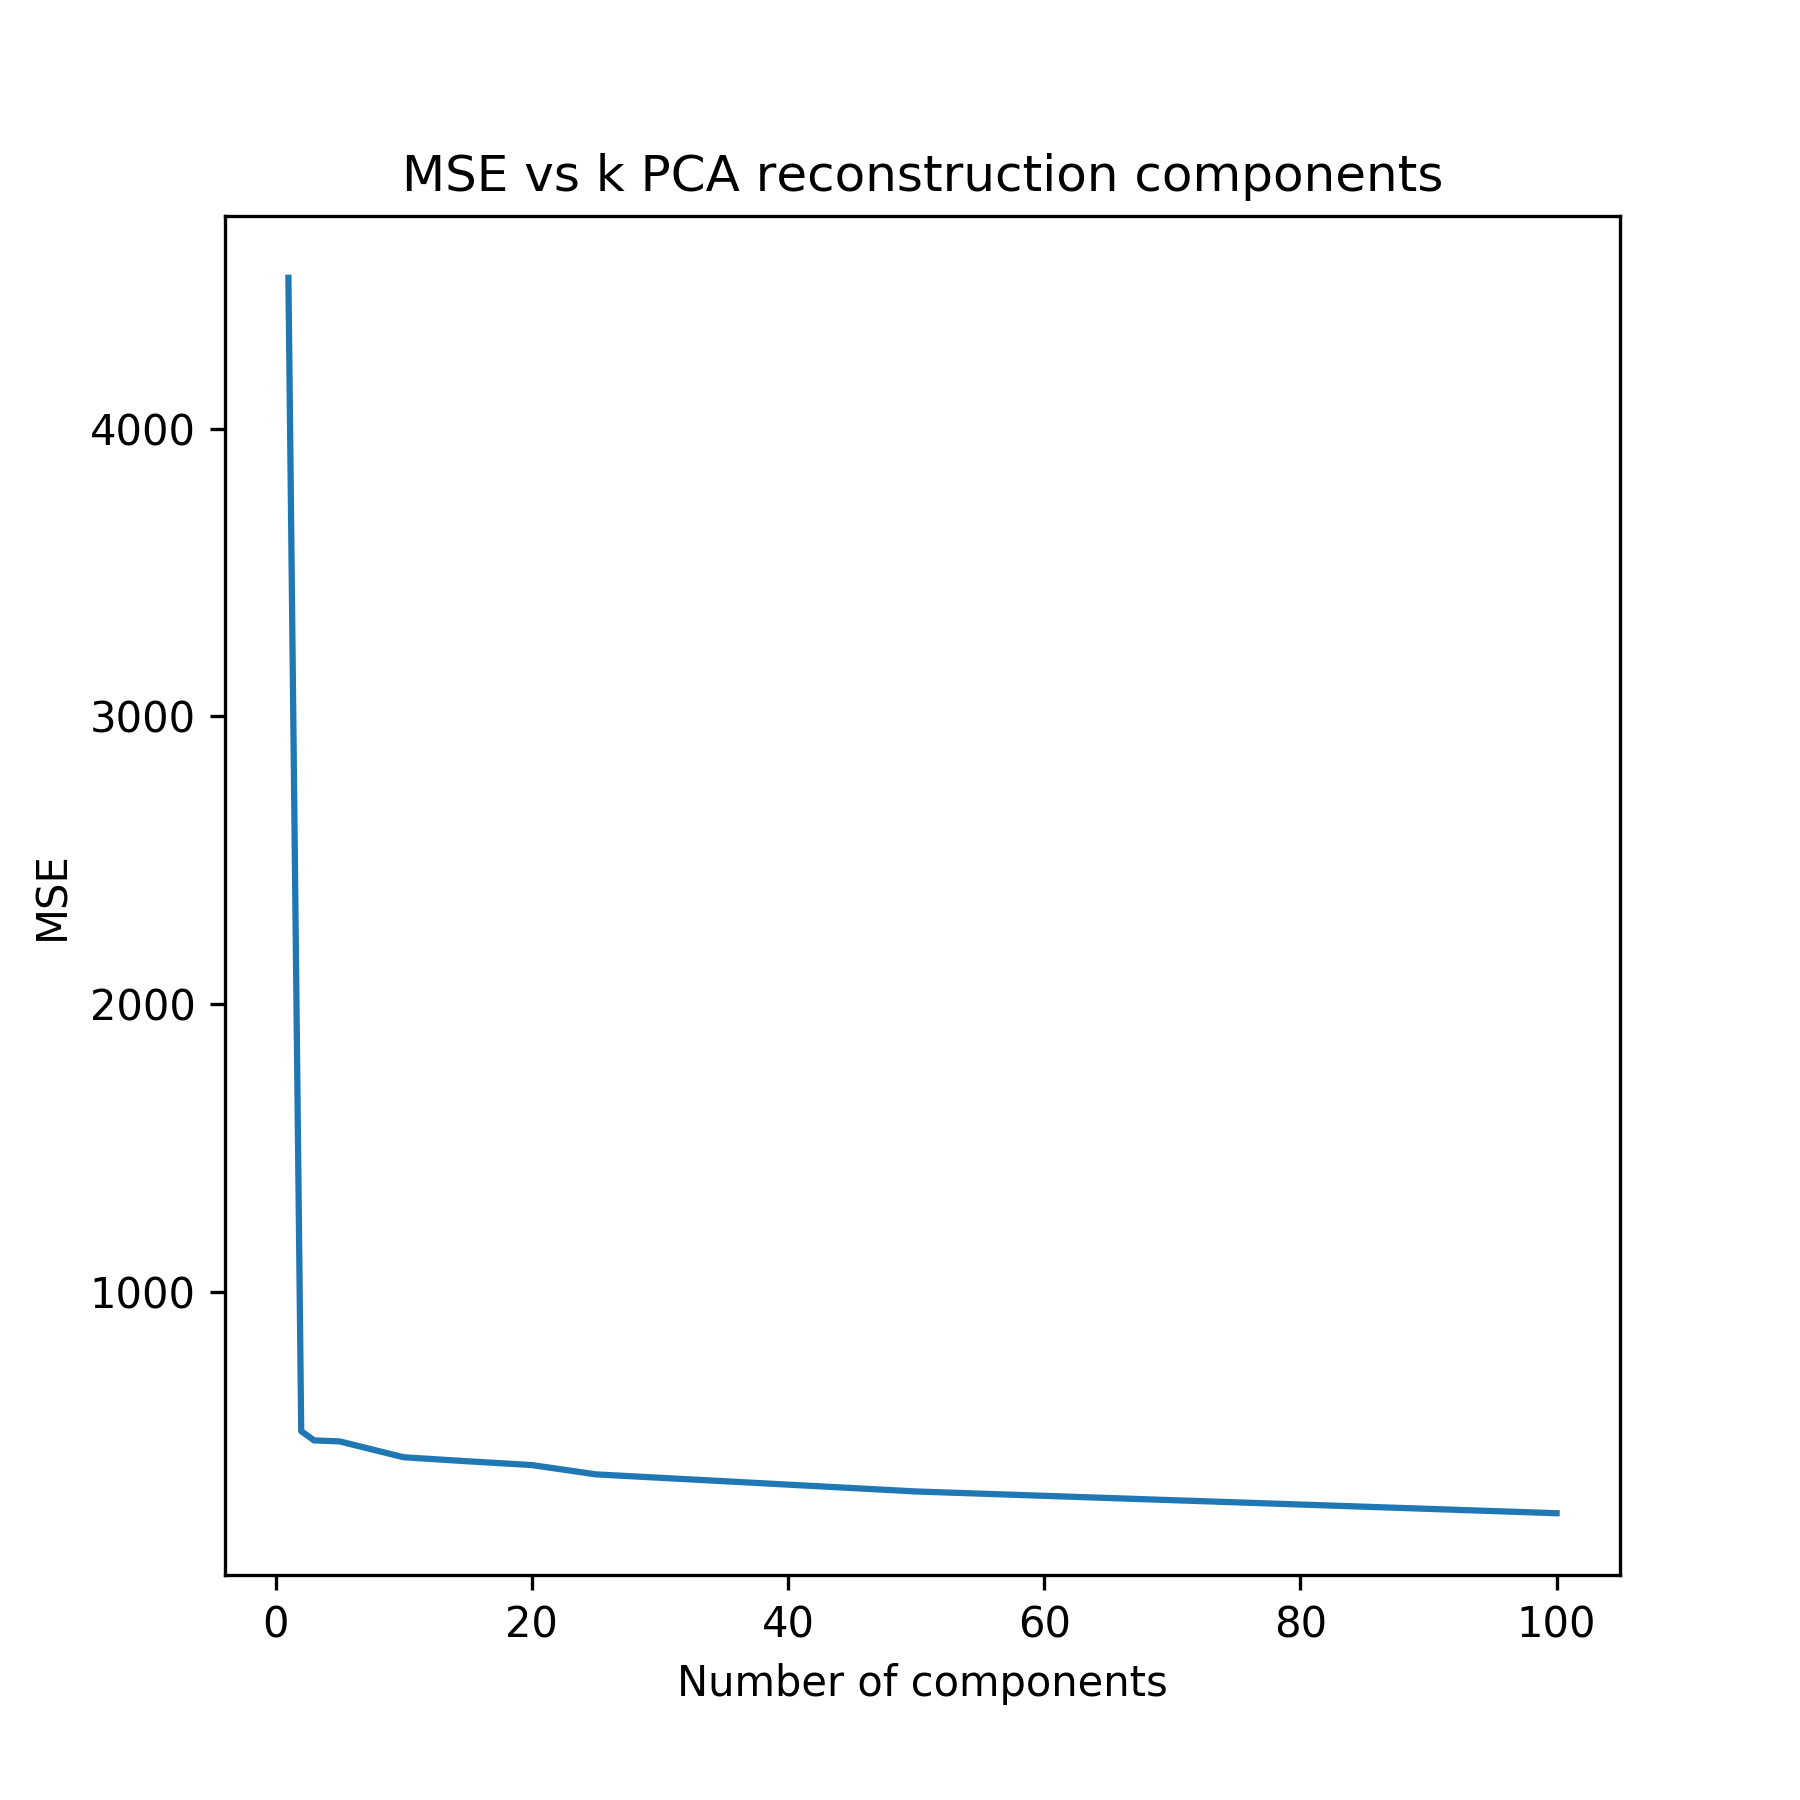
\includegraphics[width=0.7\textwidth]{../images/pca_mse_vs_k.png}
\caption{Mean-square error of PCA as number of principle components included increases.}
\label{msek}
\end{figure}

\begin{figure}
\centering
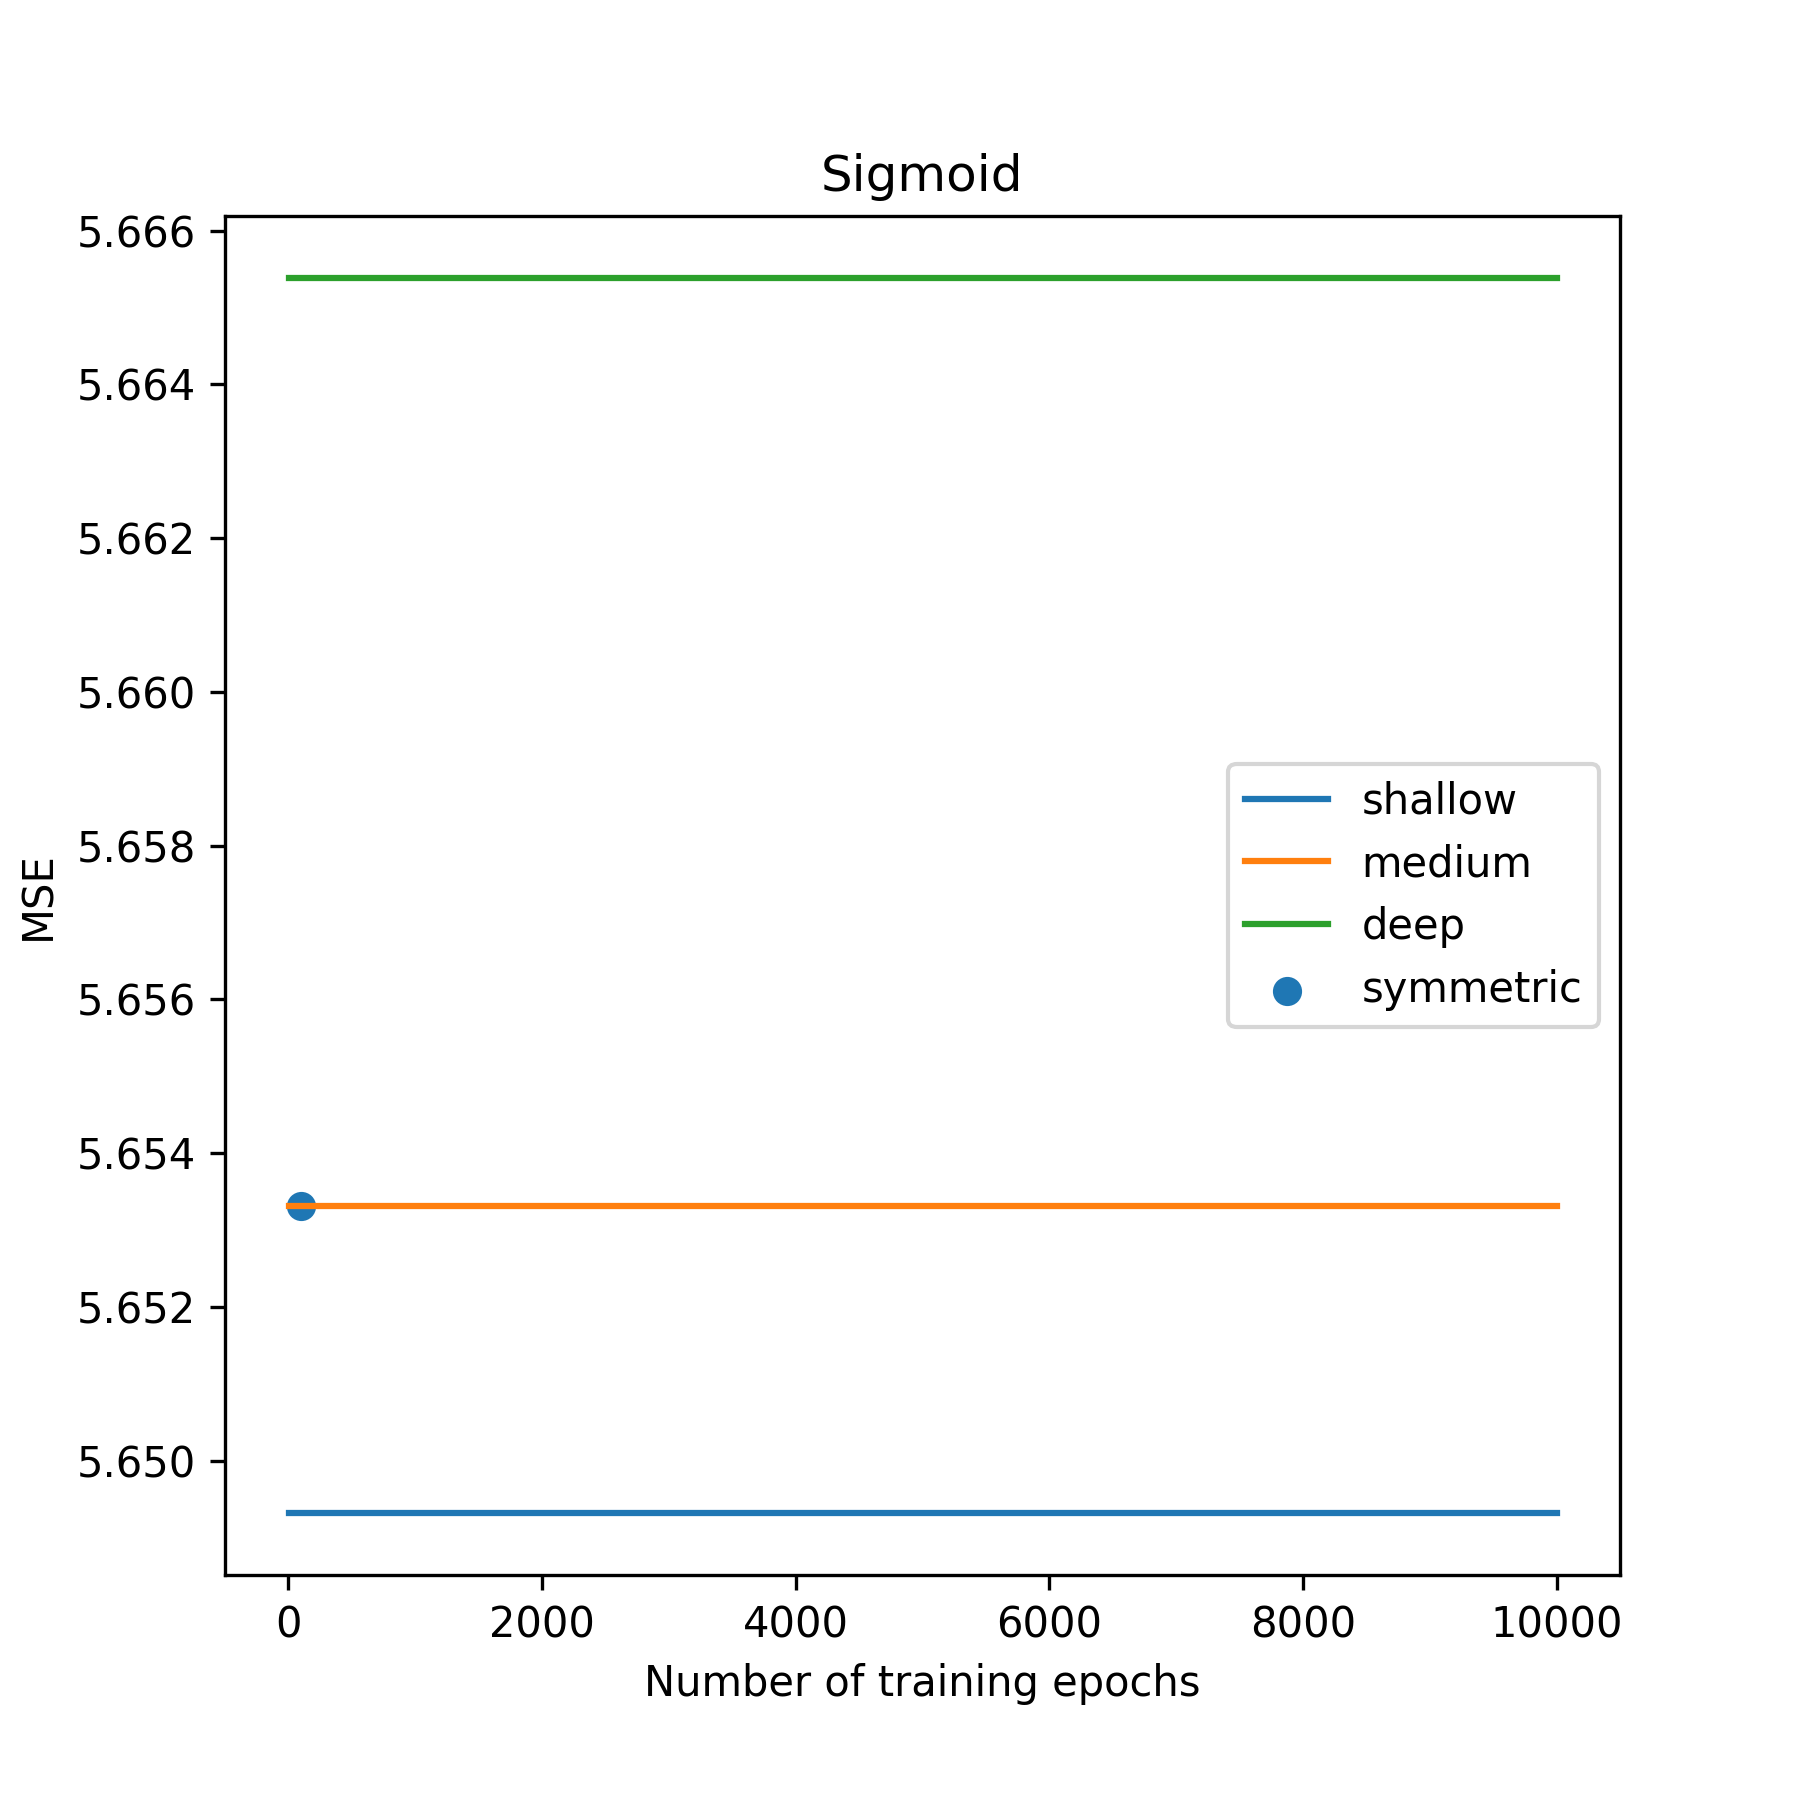
\includegraphics[width=0.7\textwidth]{../images/aenn_results_sigmoid.png}
\caption{Mean-square error of sigmoid activation AENN across training periods.}
\label{aenn_sigmoid}
\end{figure}

\begin{figure}
\centering
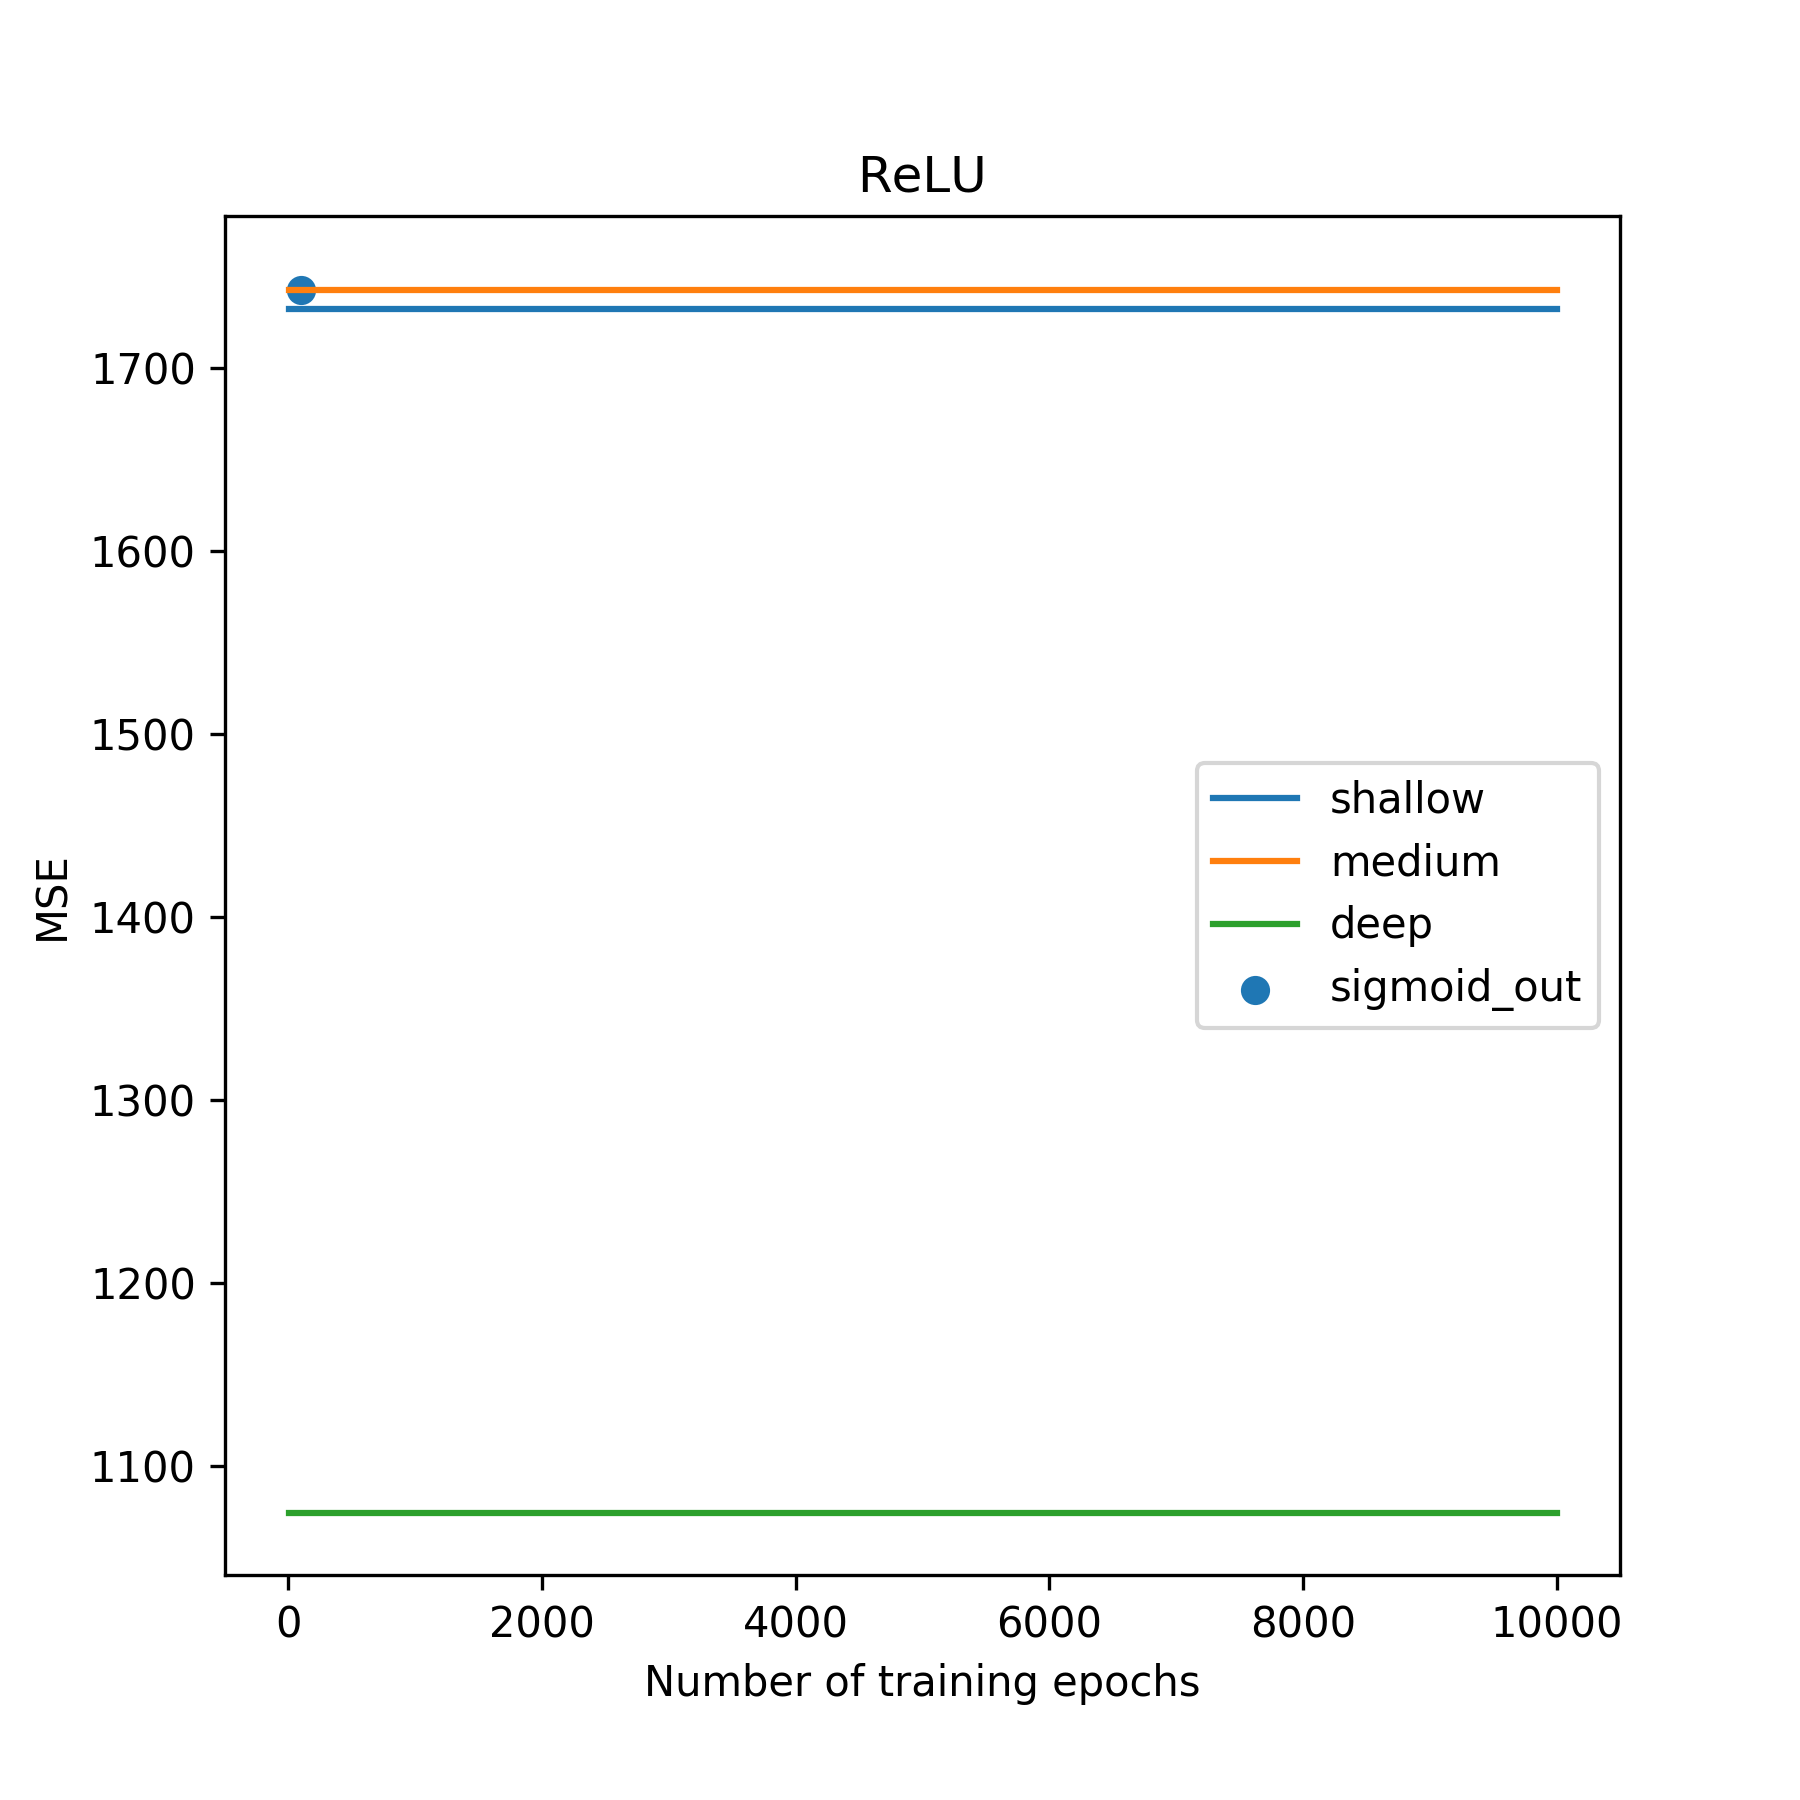
\includegraphics[width=0.7\textwidth]{../images/aenn_results_relu.png}
\caption{Mean-square error of ReLU activation AENN across training periods.}
\label{aenn_relu}
\end{figure}

\section{Conclusions}
\begin{itemize}
\item Autoencoders with logistic activation performed the best at dimensionality reduction (according to our regression mean-squared error metric), followed by regular principal-components analysis.
\item Neural networks with only ReLU activations do not perform well for dimensionality reduction, compared to other techniques we looked at.
\item For the architectures we studied, varying the number of training epochs did not change the mean-squared error. 
\item Neither combining layers with different activation functions (input and hidden ReLU and sigmoid output), nor adding symmetric decoding layers improved autoencoder performance.
\end{itemize}
\section{Future work}

There are a number of ways this work can be extended. We could use alternate encoding schemes for the free-text data, e.g. low-dimensional word embeddings produced by neural network-based algorithms such as \verb+word2vec+ or \verb+GloVe+ [8]. Additional lines of inquiry involve either different neural-network architectures, different loss functions, or alternative dimensionality reduction techniques.

We could have used regression mean-squared error as the loss function when training neural networks, but there is not a clear analog of this when doing principal-components analysis, so we opted to simply force the decoded output to be as close as possible to the unencoded input.

Further, we had hoped to compare the methods discussed to another technique called t-Distributed Stochastic Neighbor Embedding (t-SNE) [9]. Other uses of this technique, which specifically targets two- or three-dimensional representations of high-dimensional data. These techniques exist on a spectrum of stochasticity: PCA is deterministic, while autoencoders have stochastic elements, and t-SNE is completely stochastic and very sensitive to hyperparameter tuning.

\section*{References}
\small

[1] Kramer, Mark A. (1991). "Nonlinear principal component analysis using autoassociative neural networks" {\it AIChE Journal}. 37 (2): 233–243. doi:10.1002/aic.690370209.

[2] Van der Maaten, L., Postma, E. (2009). Dimensionality Reduction: A Comparative Review. {\it Accessed at \verb+https://lvdmaaten.github.io/publications/papers/TR_Dimensionality_Reduction_Review_2009.pdf+}. Last accessed Dec 19, 2019.

[3] Elden, L. (2007). {\it Matrix Methods in Data Mining and Pattern Recognition}, pp. 66. Philadelphia, PA:  Society for Industrial and Applied Mathematics.

[4] Hinton, G.E. \& Salakhutdinov, R.R. Reducing the dimensionality of data with neural networks. {\it Science}, 313(5786):504–507, 2006.

[5] Hinton GE, Krizhevsky A, Wang SD. Transforming auto-encoders. In International Conference on Artificial Neural Networks 2011 Jun 14 (pp. 44-51). Springer, Berlin, Heidelberg.

[6] Auto Encoder in Raw Numpy (2019). {\it Accessed at https://www.kaggle.com/theonenamedtoby/auto-encoder-in-raw-numpy/data}. Last accessed Dec 7, 2019.

[7] Wine Reviews (2017). {\it Accessed at https://kaggle.com/zynicide/wine-reviews}. Last accessed Dec 2, 2019.

[8] Mikolov, T., Chen, K., Corrado, G. \& Dean, J. (2013) Efficient Estimation of Word Representations in Vector Space. {\it Accessed at https://arXiv:1301.3781}. Last accessed Dec 10, 2019.

[9] L.J.P. van der Maaten and G.E. Hinton. Visualizing High-Dimensional Data Using t-SNE. Journal of Machine Learning Research 9(Nov):2579-2605, 2008.

\end{document}
